
\section{Ziel}

In diesem versuch soll die Wellenlänge eines Lasers gemessen sowie der Brechungsindex von Luft mit dem Michelson-Interferometer ermittelt werden.

\section{Theorie}

\subsection{Inteferenz und Kohärenz}
Licht kann als elektromagnetische Welle angenommen werden. Diese lässt sich mit der elektrischen Feldstärke 
\begin{equation}
  \vec E(x,t)=\vec E_{0}cos(kx-\omega t-\delta) 
  \label{koh}
\end{equation}
beschreiben, bei der x der Ort, t die Zeit, k die Wellenzahl, $\omega$ die Kreisfrequenz und $\delta$ die Phasenabweichung am Nullpunkt ist. Die Lichtwellenausbreitung lässt sich dann mit den Maxwellschen-Gleichungen beschreiben. Für jedes E-Feld gilt das Superpositionsprinzip. Da jedoch das E-Feld bei hohen Frequenzen schwer messbar ist, wird die Intensität 
\begin{equation}
  I=const|\vec E|^2 \nonumber
\end{equation}
genutzt.Insofern zwei E-Felder superponieren, kann die Intensität $I_{Ges}$ durch
\begin{equation}
  I_{Ges}=\frac{const}{t_{2}-t_{1}} \int^{t_{2}}_{t_{1}} |\vec E_{1}+\vec E_{2}|^2 (x,t)dt \nonumber
\end{equation}
berechnet werden. Damit ergibt sich 
\begin{equation}
  I_{Ges}=2const\vec E_{0}^2 (1+cos(\delta_{2}-\delta_{1})) \nonumber
\end{equation}
für den Ansatz $\vec E_{1/2}=\vec E_{0}e^{i(kx-\omega t -\delta_{1/2})}$. Hierbei ist der zweite Summand
\begin{equation}
  2const\vec E_{0}^2 cos(\delta_{2}-\delta_{1}) \nonumber
\end{equation}
der \textit{Interferenzterm}.
Die Interferenz kann konstruktiv oder destruktiv verlaufen. Sie verschwindet insofern 
\begin{equation}
  \delta_{2}-\delta_{1}=(2n+1)\pi \quad n \in \mathds{N_{0}} \nonumber
\end{equation}
ist. Allerdings ist Licht, dass aus zwei Lichtquellen stammt, nicht interferenzfähig und wird als \textit{inkohärent} bezeichnet. Deswegen muss \textit{kohärentes} Licht erzeugt werden, das mit Lasern realisierbar ist. Kohärentes Licht ist Licht, dass sich durch die Gleichung \eqref{koh} mit festem $k$, $\omega$ und $\delta$ darstellen lässt.
Wenn man das Licht mit einem Strahlteiler teilt und einen Strahl durch einen Spiegel reflektiert, sodass beide an der selben Stelle des Schirms auftreffen, wie in \autoref{fig:1}, dann sorgt die durch die Weglänge unterschiedliche Phasendifferenz für ein Interferenzmuster.
\begin{figure}[H]
  \centering
  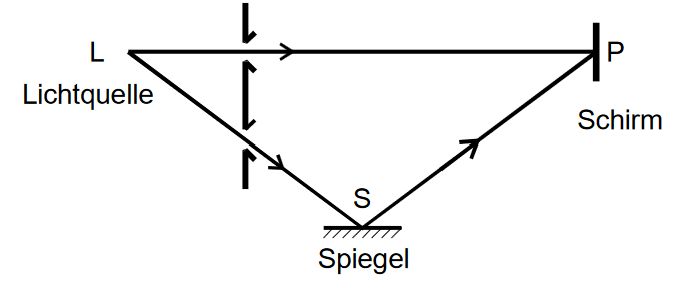
\includegraphics[width=7cm]{1}
  \caption{Mögliche Versuchsanordnung [V401]}
  \label{fig:1}
\end{figure}
Der maximale Weglängenunterschied, bei denen die Lichtstrahlen noch ein stabiles Interferenzmuster abbilden, wird \textit{Koheränzlänge} $\ell$ genannt mit
\begin{equation}
  \ell=N\lambda, \nonumber
\end{equation}
wobei N die maximal beobachteten Intensitätsmaxima auf dem Schirm sind und $\lambda$ die Wellenlänge des Lasers.

\subsection{Michelson-Interferometer}

Mit dem Michelson-Interferometer können optische Größen gemessen werden. 
\begin{figure}[H]
  \centering
  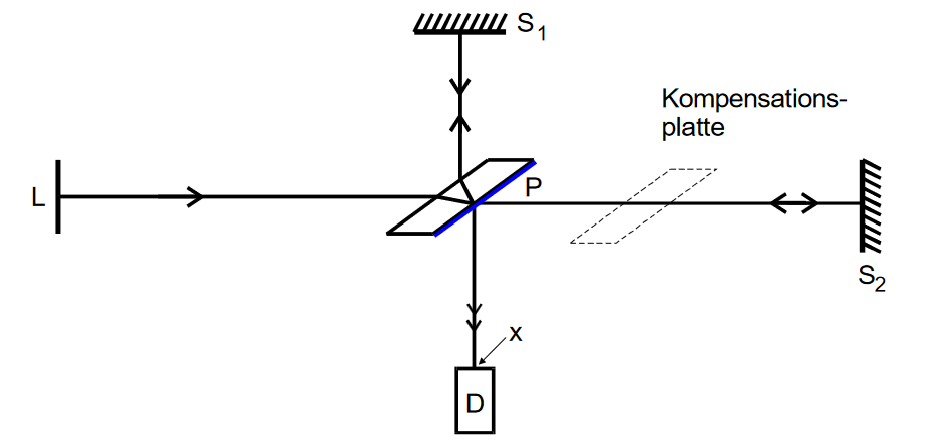
\includegraphics[width=7cm]{2}
  \caption{Aufbau des Michelson-Interferometers [V401]}
  \label{fig:2}
\end{figure}
Das Licht strahlt auf eine halbdurchlässige Platte, die einen Teil des Lichstrahls durchlässt und die andere orthogonal spiegelt. Beide Teilstrahlen treffen auf die Spiegel 1 und 2 aus \autoref{fig:2} die die Strahlen zurückreflektieren, die dann auf den Detektor fallen. Beide Strahlenbündel sind kohärent, weil $\bar{S_{1}P}=\bar{S_{2}}<\bar{LP}$ gesetzt wird. Bei $\bar{S_{1}P}=\bar{S_{2}}$ ist der Gangunterschied am Detektor $\frac{\lambda}{2}$ und die Lichtbündel inteferieren destruktiv. Wird ein Spiegel jedoch um den Weg $\Delta d$ verschoben, dann ändert sich die Intensität des Interferenzmusters am Detektor und es ergibt sich die Beziehung
\begin{equation}
  \Delta d=N\frac{\lambda}{2}
  \label{eq:1}
\end{equation}
zwischen der Verscheibung und der Wellenlänge [1].\\
Eine andere Methode den Wegunterschied zu ändern ist, das Licht durch ein Medium mit verändertem Brechungsindex zu senden. Wenn das Medium die Länge $b$ hat und der Brechungsindex sich zu $n+\Delta n$ verschiebt, ist der Wegunterschied der beiden Strahlen $b\Delta n$. Die Änderung des Brechungsindex kann durch Evakuierung einer Messbox oder Erhöhung des Drucks realisiert werden, in der sich das zu untersuchende Medium befindet. Die Beziehung \eqref{eq:1} ändert sich zu
\begin{equation}
  n\Delta n =N\frac{\lambda}{2} \nonumber
\end{equation}
und lässt sich zu 
\begin{equation}
  n=\sqrt{1+f(\lambda)N_{T}}
  \label{eq:2}
\end{equation}
umformen, mit $N_{T}$ als Anzahl von Molekülen, die durch die Lichwellen der Wellenlänge $\lambda$ angeregt wurden. Im optisch sichtbaren Bereich lässt sich \eqref{eq:2} in
\begin{equation}
  n=1+\frac{f}{2}N-... \nonumber
\end{equation}
entwickeln. Für Gase zwischen 0 und 1 Bar gilt die ideale Gasgleichung
\begin{equation}
  pV=RT 
  \label{eq:3}
\end{equation}
Um die Brechungsindexänderung $\Delta n(p,p')$ zu berechnen, wird 
\begin{equation}
  \Delta n(p,p')=f/2(N(p,T)-N(p',T))
  \label{eq:4}
\end{equation}
verwendet, bei der 
\begin{equation}
  N(p,T)=\frac{p}{T}\frac{T_{0}}{p_{0}}N_{L},\nonumber
\end{equation}
\begin{equation}
  N(p',T)=\frac{p'}{T}\frac{T_{0}}{p_{0}}N_{L}, \quad N_{L}=2,687\cdot 10^25\frac{1}{m^3}
  \label{eq:5}
\end{equation}
die Anzahl der Moleküle in Abhängigkeit des Drucks p (oder des geänderten Drucks p') und der Temperatur T ist.
Mit \eqref{eq:5} folgt aus \eqref{eq:4}
\begin{equation}
  \Delta n(p,p')=\frac{f}{2}\frac{N_{L}}{T}\frac{T_{0}}{p_{0}}(p-p') 
  \label{eq:5}
\end{equation}
und damit
\begin{equation}
  n(p_{0},T_{0})=1+\Delta n(p,p')\frac{T}{T_{0}}\frac{p_0}{p-p'},
  \label{eq:6}
\end{equation}
der Brechungsindex des Gases bei Normaldruck und -Temperatur [1].
